\documentclass[aspectratio=169]{beamer}

% ---------- ENCODING & FONTS ----------
\usepackage[utf8]{inputenc}
\usepackage[T1]{fontenc}

% ---------- THEME & LOOK ----------
\usetheme{Madrid}
\usecolortheme{seahorse}
\usefonttheme{professionalfonts}
\setbeamertemplate{navigation symbols}{}
\setbeamercovered{transparent}
\setbeamertemplate{itemize items}[circle]
\setbeamertemplate{enumerate items}[default]
\setlength{\parskip}{0.25em}

% ---------- COLORS ----------
% Beamer already loads xcolor, so we just define our colors
\definecolor{accent}{RGB}{0,92,184}
\definecolor{soft}{RGB}{233,244,255}
\definecolor{lightred}{RGB}{245,210,210}
\setbeamercolor{structure}{fg=accent}
\setbeamercolor{title}{fg=white,bg=accent}
\setbeamercolor{frametitle}{fg=accent}
\setbeamercolor{block title}{bg=accent!12,fg=accent}
\setbeamercolor{block body}{bg=soft}

% ---------- PACKAGES ----------
\usepackage{booktabs}
\usepackage{amsmath, amssymb}
\usepackage{array}
\usepackage{multirow}
\usepackage{hyperref}
\hypersetup{colorlinks=true,linkcolor=accent,urlcolor=accent}

% ---------- SAFE TRANSITION FALLBACK ----------
\makeatletter
\@ifundefined{transfade}{\newcommand{\transfade}[1][]{}}{}
\makeatother

% ---------- PLACEHOLDER BOX FOR FIGURES ----------
\newcommand{\placeholderbox}[2][0.82\linewidth]{%
  \begin{center}
    \fbox{\begin{minipage}[c][0.46\textheight][c]{#1}
      \centering \vspace{0.3em}
      \textbf{#2}\\[0.6em]
      \emph{Insert figure/diagram here later.}
    \end{minipage}}
  \end{center}
}

% ---------- TITLE ----------
\title{\textbf{Unemployment and Inflation \vspace{.5cm}\\  }}
\subtitle{ {\large ECON 101 - Macroeconomics}}
%\institute{UNBC}
\author{Muhebullah Karimzada}
\date{Winter 2026}



\begin{document}

% ============================================================
% TITLE
% ============================================================
\begin{frame}[plain]
  \titlepage
\end{frame}

% ============================================================
\begin{frame}{Chapter Outline}
\transfade
\begin{itemize}[<+->]
  \item \textbf{5.1} Measuring the Unemployment Rate and the Labour Force Participation Rate
  \item \textbf{5.2} Types of Unemployment
  \item \textbf{5.3} Explaining Unemployment
  \item \textbf{5.4} Measuring Inflation
  \item \textbf{5.5} Using Price Indexes to Adjust for the Effects of Inflation
  \item \textbf{5.6} Real versus Nominal Interest Rates
  \item \textbf{5.7} Does Inflation Impose Costs on the Economy?
\end{itemize}
\end{frame}

% ============================================================
\section*{Why Unemployment and Inflation Matter}
% ============================================================

\begin{frame}{Measuring Unemployment and Inflation}
\transfade
\begin{itemize}[<+->]
  \item Previous chapter: how to measure \textbf{total output} (GDP).
  \item This chapter: how to measure
  \begin{itemize}[<+->]
    \item \textbf{Unemployment} in the labour market, and
    \item \textbf{Inflation} in the goods and services market.
  \end{itemize}
  \item Both are central for:
  \begin{itemize}[<+->]
    \item macroeconomic policy,
    \item evaluating economic performance,
    \item everyday decisions of households and firms.
  \end{itemize}
\end{itemize}
\end{frame}

% ============================================================
\section{5.1 Measuring the Unemployment Rate and Labour Force Participation}
% ============================================================

\begin{frame}{5.1 Learning Objective}
\transfade
\begin{block}{Goal}
Understand how unemployment, labour force participation, and employment rates are measured.
\end{block}
\begin{itemize}[<+->]
  \item Canada is a large economy – millions of people, changing jobs all the time.
  \item We cannot track every person individually in real time.
  \item Instead, Statistics Canada uses \textbf{survey data} to estimate:
  \begin{itemize}[<+->]
    \item employment,
    \item unemployment,
    \item labour force participation,
    \item employment-population ratio.
  \end{itemize}
\end{itemize}
\end{frame}

\begin{frame}{The Labour Force and Unemployment}
\transfade
\begin{itemize}[<+->]
  \item \textbf{Labour force:} sum of \alert{employed} and \alert{unemployed} workers in the economy.
  \item \textbf{Unemployment rate:} percentage of the labour force that is unemployed:
  \[
    \text{Unemployment rate} = 
    \frac{\text{Number of unemployed}}{\text{Labour force}} \times 100.
  \]
  \item These are monthly headline numbers often reported in the news.
\end{itemize}
\end{frame}

\begin{frame}{The Labour Force Survey (LFS)}
\transfade
\begin{itemize}[<+->]
  \item Each month, Statistics Canada conducts the \textbf{Labour Force Survey (LFS)}.
  \item Roughly \textbf{56,000 households} are selected to be representative.
  \item Members of \textbf{working age} (15 years and older) are:
  \begin{itemize}[<+->]
    \item asked about employment status, and
    \item asked about recent \textbf{job search} activities.
  \end{itemize}
  \item Based on the answers, each person is classified as:
  \begin{itemize}[<+->]
    \item \textbf{Employed}
    \item \textbf{Unemployed}
    \item \textbf{Not in the labour force}
  \end{itemize}
\end{itemize}
\end{frame}

\begin{frame}{Definitions: Employed, Unemployed, Not in the Labour Force}
\transfade
\begin{itemize}[<+->]
  \item \textbf{Employed:}
  \begin{itemize}[<+->]
    \item Did paid work, or
    \item Did unpaid work for a family business, or
    \item Worked for themselves, or
    \item Were temporarily away from their jobs (vacation, illness, strike).
  \end{itemize}
  \item \textbf{Unemployed:}
  \begin{itemize}[<+->]
    \item Not currently at work,
    \item \emph{Available} for work,
    \item Actively looked for work in the previous four weeks.
  \end{itemize}
  \item \textbf{Not in the labour force:}
  \begin{itemize}[<+->]
    \item Neither employed nor unemployed (students not seeking work, retirees, etc.).
  \end{itemize}
\end{itemize}
\end{frame}

\begin{frame}{Figure 5.1 -- Employment Status of the Working-Age Population}
\centering


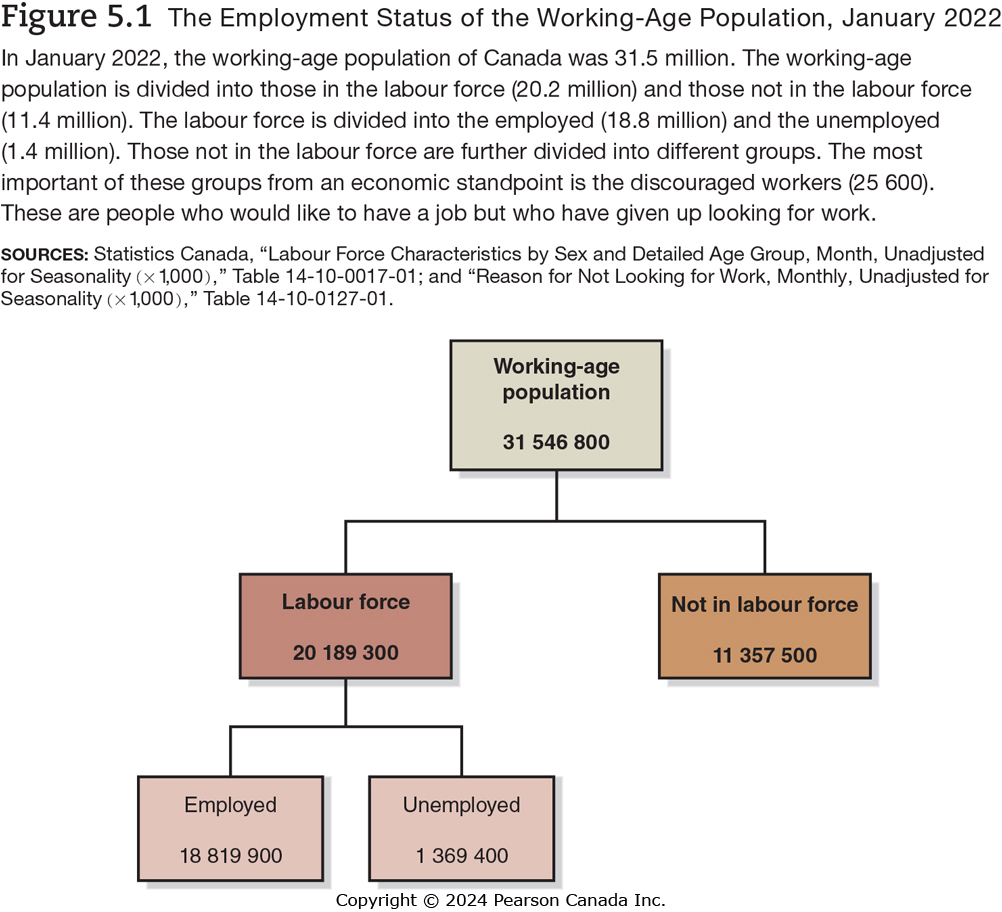
\includegraphics[width=0.71\linewidth]{Fig05-001}.
\end{frame}

\begin{frame}{Labour Force Participation Rate}
\transfade
\begin{itemize}[<+->]
  \item \textbf{Labour force participation rate:}
  \[
    \text{LFPR} = 
    \frac{\text{Labour force}}{\text{Working-age population}} \times 100.
  \]
  \item Measures what fraction of working-age people are \textbf{actively} in the labour market.
  \item Helps us distinguish:
  \begin{itemize}[<+->]
    \item low unemployment because people have jobs,
    \item vs.\ low unemployment because many have given up looking for work.
  \end{itemize}
\end{itemize}
\end{frame}

\begin{frame}{Employment-Population Ratio}
\transfade
\begin{itemize}[<+->]
  \item \textbf{Employment-population ratio:}
  \[
    \text{Employment-population ratio} =
    \frac{\text{Number employed}}{\text{Working-age population}} \times 100.
  \]
  \item This tells us how many people \textbf{actually have jobs}, relative to the working-age population.
  \item Useful indicator of the \textbf{health of the labour market} during expansions and recessions.
\end{itemize}
\end{frame}



\begin{frame}{Problems with Measuring the Unemployment Rate}
\transfade
\begin{itemize}[<+->]
  \item The measured unemployment rate is \textbf{not perfect}.
  \item It may \alert{understate} true unemployment:
  \begin{itemize}[<+->]
    \item Distinguishing between \textbf{unemployed} and \textbf{not in the labour force} can be difficult.
    \item \textbf{Discouraged workers}: people who have stopped looking for work but would take a job if offered one.
    \item It does not measure intensity of employment — e.g., part-time vs.\ full-time, underemployment.
  \end{itemize}
  \item It may \alert{overstate} unemployment:
  \begin{itemize}[<+->]
    \item Some people may claim to be unemployed while not seriously looking, to keep benefits or avoid taxes.
  \end{itemize}
\end{itemize}
\end{frame}

\begin{frame}{Figure 5.2 -- Trends in Labour Force Participation}
\centering


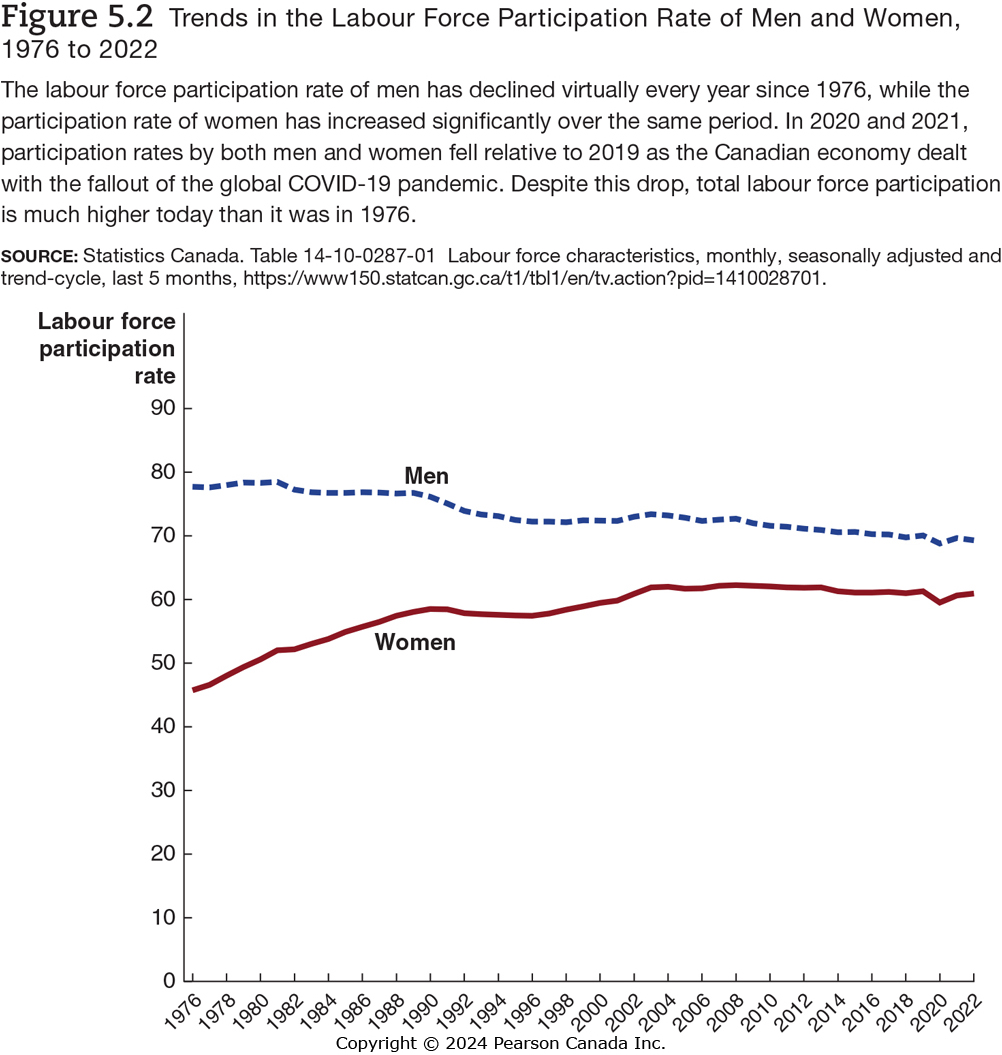
\includegraphics[width=0.65\linewidth]{Fig05-002}.
\end{frame}


\begin{frame}{Job Creation and Job Destruction}
\transfade
\begin{itemize}[<+->]
  \item The labour market is \textbf{dynamic}:
  \begin{itemize}[<+->]
    \item Firms constantly create and destroy jobs.
  \end{itemize}
  \item Example (from the slide):
  \begin{itemize}[<+->]
    \item In January 2022, there were 890,500 more people employed than in January 2021.
    \item But the number of jobs \textbf{created} was much larger, because many jobs were also \textbf{destroyed}.
  \end{itemize}
  \item Month to month, some provinces can see large job losses even while the national economy is improving.
\end{itemize}
\end{frame}

% ============================================================
\section{5.2 Types of Unemployment}
% ============================================================

\begin{frame}{5.2 Learning Objective}
\transfade
\begin{block}{Goal}
Identify and understand the four types of unemployment.
\end{block}
\begin{itemize}[<+->]
  \item Unemployment is not a single phenomenon.
  \item To interpret unemployment correctly, we distinguish:
  \begin{itemize}[<+->]
    \item frictional,
    \item structural,
    \item cyclical,
    \item seasonal unemployment.
  \end{itemize}
\end{itemize}
\end{frame}

\begin{frame}{Figure 5.3 -- The Unemployment Rate in Canada }
\centering


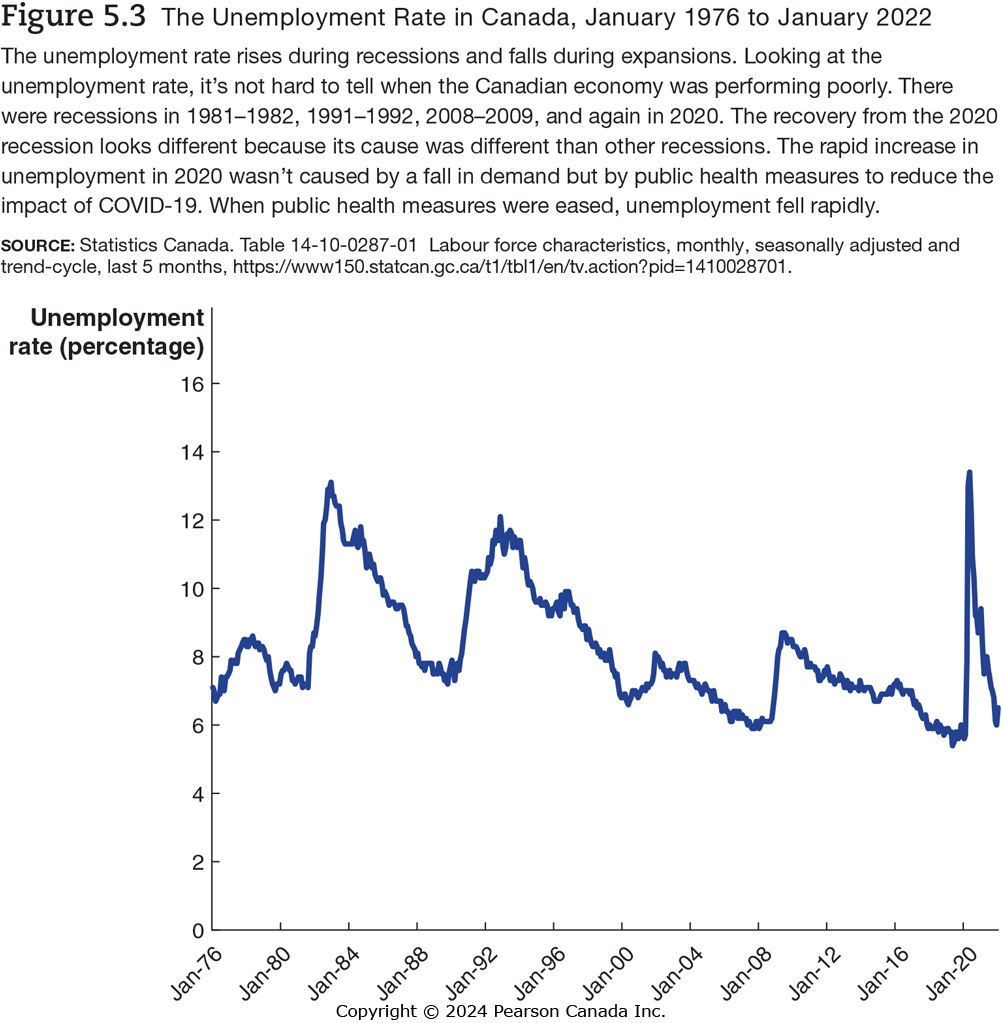
\includegraphics[width=0.65\linewidth]{Fig05-003}.
\end{frame}

\begin{frame}{Four Types of Unemployment}
\transfade
\begin{itemize}[<+->]
  \item \textbf{Frictional unemployment}
  \item \textbf{Structural unemployment}
  \item \textbf{Cyclical unemployment}
  \item \textbf{Seasonal unemployment}
  \item Each type has different causes and different policy implications.
\end{itemize}
\end{frame}

\begin{frame}{Frictional Unemployment}
\transfade
\begin{itemize}[<+->]
  \item \textbf{Frictional unemployment:}
  \begin{itemize}[<+->]
    \item Short-term unemployment that arises from the process of matching workers with jobs.
  \end{itemize}
  \item Mainly due to \textbf{job search}:
  \begin{itemize}[<+->]
    \item People entering or re-entering the labour force.
    \item People between jobs.
  \end{itemize}
  \item Some frictional unemployment is \alert{unavoidable}:
  \begin{itemize}[<+->]
    \item People need time to learn about opportunities and find good matches.
  \end{itemize}
  \item In fact, some frictional unemployment can \alert{increase} economic efficiency:
  \begin{itemize}[<+->]
    \item It allows workers to find jobs that better fit their skills and preferences.
  \end{itemize}
\end{itemize}
\end{frame}

\begin{frame}{Example: Frictional Unemployment}
\transfade
\begin{itemize}[<+->]
  \item A recent university graduate spends three months searching for a job in their field.
  \item They are counted as \textbf{unemployed}, but this is frictional unemployment.
  \item From the economy’s perspective:
  \begin{itemize}[<+->]
    \item It is better for them to search a bit longer and find a suitable, productive job than to accept the first random job.
  \end{itemize}
\end{itemize}
\end{frame}

\begin{frame}{Structural Unemployment}
\transfade
\begin{itemize}[<+->]
  \item \textbf{Structural unemployment:}
  \begin{itemize}[<+->]
    \item Unemployment that arises from a persistent \alert{mismatch} between the skills and attributes of workers and the requirements of jobs.
  \end{itemize}
  \item Often associated with:
  \begin{itemize}[<+->]
    \item technological change,
    \item changes in demand for certain industries,
    \item regional shifts in economic activity.
  \end{itemize}
  \item Structural unemployment tends to be \textbf{longer-term}:
  \begin{itemize}[<+->]
    \item Workers may need retraining or relocation.
  \end{itemize}
\end{itemize}
\end{frame}

\begin{frame}{Example: Structural Unemployment}
\transfade
\begin{itemize}[<+->]
  \item A manufacturing worker loses their job due to automation.
  \item Their skills do not easily transfer to growing sectors such as IT or health care.
  \item Without retraining, they may remain unemployed for a long period.
\end{itemize}
\end{frame}

\begin{frame}{Cyclical Unemployment}
\transfade
\begin{itemize}[<+->]
  \item \textbf{Cyclical unemployment:}
  \begin{itemize}[<+->]
    \item Unemployment caused by a \alert{business cycle recession}.
  \end{itemize}
  \item When aggregate demand falls:
  \begin{itemize}[<+->]
    \item firms reduce output,
    \item and lay off workers even if workers are skilled and jobs are otherwise a good match.
  \end{itemize}
  \item Example:
  \begin{itemize}[<+->]
    \item In February 2009, Chrysler temporarily closed its assembly plant in Brampton, Ontario, due to low sales.
    \item Laid-off employees experienced \textbf{cyclical unemployment}.
  \end{itemize}
\end{itemize}
\end{frame}

\begin{frame}{Seasonal Unemployment}
\transfade
\begin{itemize}[<+->]
  \item \textbf{Seasonal unemployment:}
  \begin{itemize}[<+->]
    \item Unemployment due to seasonal factors such as weather or calendar patterns.
  \end{itemize}
  \item Examples:
  \begin{itemize}[<+->]
    \item Construction and tourism often slow in winter.
    \item Agriculture, fisheries, and some retail sectors are highly seasonal.
  \end{itemize}
  \item Seasonal unemployment can make the measured unemployment rate:
  \begin{itemize}[<+->]
    \item artificially high in winter,
    \item artificially low in summer.
  \end{itemize}
  \item To address this, Statistics Canada provides:
  \begin{itemize}[<+->]
    \item \textbf{seasonally adjusted} series (seasonal effects removed),
    \item \textbf{unadjusted} series (seasonal effects included).
  \end{itemize}
\end{itemize}
\end{frame}

\begin{frame}{Full Employment and the Natural Rate of Unemployment}
\transfade
\begin{itemize}[<+->]
  \item Even in good times, there is always some unemployment.
  \item When all unemployment is due to frictional and structural factors, the economy is at \textbf{full employment}.
  \item \textbf{Natural rate of unemployment:}
  \begin{itemize}[<+->]
    \item The normal rate of unemployment, consisting of frictional and structural unemployment.
  \end{itemize}
  \item Estimates for Canada suggest a natural rate around \textbf{5.6--6.7\%} in recent years.
\end{itemize}
\end{frame}

% ============================================================
\section{5.3 Explaining Unemployment}
% ============================================================

\begin{frame}{5.3 Learning Objective}
\transfade
\begin{block}{Goal}
Explain what determines the unemployment rate and how policy affects it.
\end{block}
\begin{itemize}[<+->]
  \item Governments often try to influence unemployment directly and indirectly.
  \item Some policies \alert{reduce} frictional or structural unemployment.
  \item Other policies can unintentionally \alert{increase} unemployment.
\end{itemize}
\end{frame}

\begin{frame}{Government Policies and Unemployment}
\transfade
\begin{itemize}[<+->]
  \item Examples of policies that can \textbf{reduce unemployment}:
  \begin{itemize}[<+->]
    \item Retraining programs (e.g., Ontario’s “Better Jobs Ontario”) to reduce structural unemployment.
    \item Hiring subsidies or job search assistance to reduce frictional unemployment.
  \end{itemize}
  \item Examples of policies that might \textbf{increase unemployment}:
  \begin{itemize}[<+->]
    \item Employment insurance (if very generous),
    \item Minimum wage laws that raise the cost of hiring,
    \item Some labour market regulations.
  \end{itemize}
\end{itemize}
\end{frame}

\begin{frame}{Employment Insurance (EI)}
\transfade
\begin{itemize}[<+->]
  \item Suppose you lose your job. You can:
  \begin{itemize}[<+->]
    \item take a new low-paying job immediately, or
    \item search for a better job that matches your skills.
  \end{itemize}
  \item If \textbf{employment insurance} payments are available, you are more likely to choose the second option.
  \item In Canada, EI replaces about \textbf{55\%} of earnings up to a weekly maximum (e.g., \$595 per week in 2021).
  \item EI effects:
  \begin{itemize}[<+->]
    \item Allows more time for job search \(\Rightarrow\) better matches, higher productivity.
    \item But also tends to \alert{increase} the average duration of unemployment.
  \end{itemize}
\end{itemize}
\end{frame}

\begin{frame}{Minimum Wage Laws}
\transfade
\begin{itemize}[<+->]
  \item Minimum wage laws are designed to help low-income workers.
  \item Raising the minimum wage increases the \textbf{cost of labour}.
  \item Firms may respond by:
  \begin{itemize}[<+->]
    \item hiring fewer workers,
    \item substituting capital for labour,
    \item reducing hours.
  \end{itemize}
  \item In Canada, minimum wages vary by province:
\end{itemize}
\small
\begin{tabular}{l c}
\toprule
Region & Example Minimum Wage (June 2022) \\
\midrule
Nunavut & \$16.00/hour \\
New Brunswick & \$12.75/hour \\
\bottomrule
\end{tabular}

\vspace{0.4em}
\begin{itemize}[<+->]
  \item Studies suggest a 10\% increase in the minimum wage might reduce teenage employment by about 2\%.
  \item Overall effect on total unemployment is believed to be \textbf{relatively small}.
\end{itemize}
\end{frame}

\begin{frame}{Labour Unions}
\transfade
\begin{itemize}[<+->]
  \item \textbf{Labour unions:} organizations of workers that bargain with employers for:
  \begin{itemize}[<+->]
    \item higher wages,
    \item better working conditions.
  \end{itemize}
  \item Unions can push wages above the competitive level for their members.
  \item In Canada:
  \begin{itemize}[<+->]
    \item about \textbf{30.9\%} of workers belonged to a union by the end of 2021,
    \item roughly \textbf{77.2\%} of government employees are unionized,
    \item only about \textbf{15.3\%} of private-sector workers are unionized.
  \end{itemize}
  \item Conclusion: unions likely have \textbf{limited impact} on overall unemployment in Canada.
\end{itemize}
\end{frame}

\begin{frame}{Efficiency Wages}
\transfade
\begin{itemize}[<+->]
  \item \textbf{Efficiency wage:} a wage above the market-clearing level that firms pay to increase workers’ productivity.
  \item Why pay more than necessary?
  \begin{itemize}[<+->]
    \item Higher wages can reduce worker turnover.
    \item They can increase effort and reduce shirking.
    \item They can attract higher-quality applicants.
  \end{itemize}
  \item But paying an efficiency wage means:
  \begin{itemize}[<+->]
    \item firms hire fewer workers,
    \item some workers who want jobs at that wage cannot find them.
  \end{itemize}
  \item This contributes to \textbf{persistent unemployment}, even when the economy is not in recession.
\end{itemize}
\end{frame}

% ============================================================
\section{5.4 Measuring Inflation}
% ============================================================

\begin{frame}{5.4 Learning Objective}
\transfade
\begin{block}{Goal}
Define the price level and inflation rate, and understand how they are computed.
\end{block}
\begin{itemize}[<+->]
  \item We introduced the \textbf{price level} in the previous chapter using the GDP deflator.
  \item Now we look at more detailed measures used in practice:
  \begin{itemize}[<+->]
    \item the \textbf{Consumer Price Index (CPI)},
    \item the \textbf{Producer Price Index (PPI)}.
  \end{itemize}
\end{itemize}
\end{frame}

\begin{frame}{Price Level and Inflation Rate}
\transfade
\begin{itemize}[<+->]
  \item \textbf{Price level:} a measure of the average prices of goods and services in the economy.
  \item \textbf{Inflation rate:} the percentage increase in the price level from one year to the next:
  \[
    \text{Inflation rate} =
    \frac{\text{Price level}_t - \text{Price level}_{t-1}}
         {\text{Price level}_{t-1}} \times 100.
  \]
  \item In Chapter 4, we used the \textbf{GDP deflator} to measure the price level for all final goods and services.
  \item However, households and firms are often more interested in specific baskets of goods.
\end{itemize}
\end{frame}

\begin{frame}{The Consumer Price Index (CPI)}
\transfade
\begin{itemize}[<+->]
  \item \textbf{CPI:} measures the average change over time in the prices paid by a typical household for the goods and services they purchase.
  \item It is based on a fixed \textbf{basket of goods and services}.
  \item Example categories:
  \begin{itemize}[<+->]
    \item food, shelter, transportation, clothing, recreation, etc.
  \end{itemize}
  \item CPI is widely used to:
  \begin{itemize}[<+->]
    \item index wages,
    \item adjust pensions and benefits,
    \item compare the cost of living over time.
  \end{itemize}
\end{itemize}
\end{frame}

\begin{frame}{Figure 5.4 -- The CPI Basket}
\centering


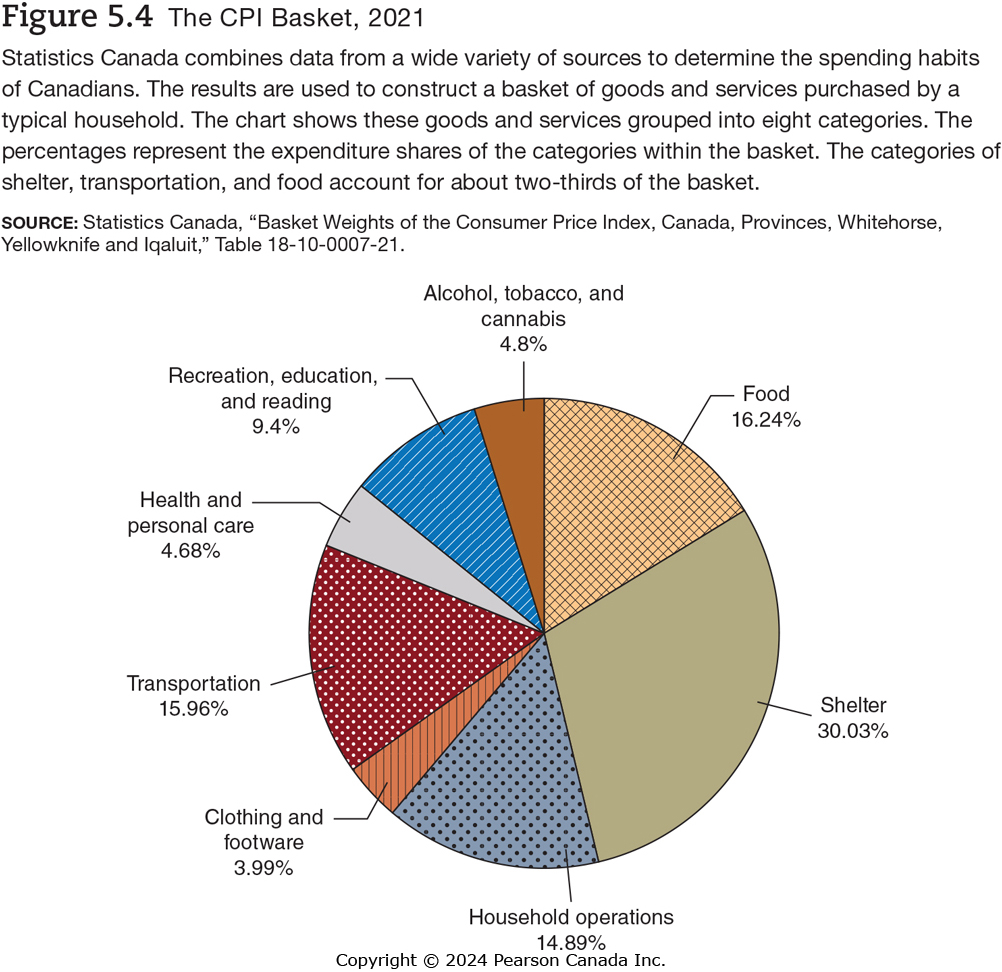
\includegraphics[width=0.62\linewidth]{Fig05-004}.
\end{frame}

\begin{frame}{Calculating the CPI}
\transfade
\begin{itemize}[<+->]
  \item To compute the CPI for a given year, we need:
  \begin{itemize}[<+->]
    \item A fixed \textbf{basket of goods and services} (quantities from a base year).
    \item The cost of buying the basket in the \textbf{base year}.
    \item The cost of buying the basket in the \textbf{current year}.
  \end{itemize}
  \item Then:
  \[
    \text{CPI}_t = 
    \frac{\text{Cost of basket in year } t}{\text{Cost of basket in base year}} \times 100.
  \]
  \item By convention, \(\text{CPI}_{\text{base year}} = 100\).
\end{itemize}
\end{frame}

\begin{frame}{A Simple CPI Calculation (1 of 2)}
\transfade
\begin{itemize}[<+->]
  \item Suppose the CPI basket (from 2002) has:
  \begin{itemize}[<+->]
    \item 10 units of good A,
    \item 5 units of good B,
    \item 2 units of good C.
  \end{itemize}
  \item We know prices for 2002, 2022, and 2023 from the slide table.
  \item \textbf{Cost of basket in 2002:}
  \[
    \text{Cost}_{2002} = 
    10 P_A^{2002} + 5 P_B^{2002} + 2 P_C^{2002}.
  \]
\end{itemize}
\end{frame}

\begin{frame}{A Simple CPI Calculation (2 of 2)}
\transfade
\begin{itemize}[<+->]
  \item \textbf{Cost of basket in 2022:}
  \[
    \text{Cost}_{2022} = 
    10 P_A^{2022} + 5 P_B^{2022} + 2 P_C^{2022}.
  \]
  \item \textbf{CPI in 2022:}
  \[
    \text{CPI}_{2022} = 
    \frac{\text{Cost}_{2022}}{\text{Cost}_{2002}} \times 100.
  \]
  \item Similarly for 2023.
  \item \textbf{Inflation between 2022 and 2023:}
  \[
    \text{Inflation} = 
    \frac{\text{CPI}_{2023} - \text{CPI}_{2022}}{\text{CPI}_{2022}} \times 100.
  \]
  \item This inflation rate is often called \textbf{CPI inflation} or a \textbf{cost-of-living} measure.
\end{itemize}
\end{frame}

\begin{frame}{Apply the Concept: Were Prices Really Cheaper in the Past?}
\transfade
\begin{itemize}[<+->]
  \item Example from the slides:
  \begin{itemize}[<+->]
    \item In 1915, a pair of cashmere socks cost \$0.35.
    \item In 2021, a similar pair costs \$39.00.
  \end{itemize}
  \item Nominally, socks are much more expensive today.
  \item But incomes are also much higher.
  \item Using the CPI to convert \$0.35 (1915) into 2021 dollars gives about \$8.13.
  \item Compared with the actual 2021 price of \$39, socks are more expensive in real terms, but relative to \textbf{average income}, households today can afford many more socks than in the past.
\end{itemize}
\end{frame}

\begin{frame}{Is the CPI Accurate?}
\transfade
\begin{itemize}[<+->]
  \item The CPI is widely used, but it is not perfect.
  \item Four main biases:
  \begin{itemize}[<+->]
    \item \textbf{Substitution bias}
    \item \textbf{Increase in quality bias}
    \item \textbf{New product bias}
    \item \textbf{Outlet bias}
  \end{itemize}
  \item Together, these biases tend to make CPI inflation \alert{overstate} the true increase in the cost of living (by about 0.5 to 1 percentage point per year).
\end{itemize}
\end{frame}

\begin{frame}{CPI Biases in More Detail}
\transfade
\begin{itemize}[<+->]
  \item \textbf{Substitution bias:}
  \begin{itemize}[<+->]
    \item Basket is fixed; in reality, consumers substitute toward relatively cheaper goods.
  \end{itemize}
  \item \textbf{Quality change bias:}
  \begin{itemize}[<+->]
    \item Part of the price increase reflects better quality (e.g., safer, more efficient cars).
  \end{itemize}
  \item \textbf{New product bias:}
  \begin{itemize}[<+->]
    \item New goods (e.g., smartphones, tablets) enter the basket with a delay.
  \end{itemize}
  \item \textbf{Outlet bias:}
  \begin{itemize}[<+->]
    \item Shift from traditional stores to discount outlets or online retailers is not fully captured by the fixed basket.
  \end{itemize}
\end{itemize}
\end{frame}

\begin{frame}{Producer Price Index (PPI)}
\transfade
\begin{itemize}[<+->]
  \item \textbf{PPI:} an average of the prices received by producers of goods and services at all stages of production.
  \item Uses a basket of:
  \begin{itemize}[<+->]
    \item raw materials,
    \item intermediate goods,
    \item goods sold by wholesalers.
  \end{itemize}
  \item Changes in the PPI often signal future movements in consumer prices:
  \begin{itemize}[<+->]
    \item higher input costs today tend to lead to higher retail prices later.
  \end{itemize}
\end{itemize}
\end{frame}

% ============================================================
\section{5.5 Using Price Indexes to Adjust for Inflation}
% ============================================================

\begin{frame}{5.5 Learning Objective}
\transfade
\begin{block}{Goal}
Use price indexes to adjust nominal values for inflation.
\end{block}
\begin{itemize}[<+->]
  \item Often we want to compare \textbf{purchasing power} across years.
  \item To do this, we convert nominal amounts into \textbf{real} amounts using a price index like the CPI.
\end{itemize}
\end{frame}

\begin{frame}{Adjusting Nominal Values for Inflation}
\transfade
\begin{itemize}[<+->]
  \item Suppose your mother earned \$30,000 in 1993.
  \item \$30,000 in 1993 could buy more goods and services than \$30,000 in 2021.
  \item To express the 1993 salary in 2021 dollars:
  \[
    \text{Value in 2021 dollars} =
    \text{Value in 1993 dollars} \times
    \frac{\text{CPI}_{2021}}{\text{CPI}_{1993}}.
  \]
  \item Using the actual CPI numbers from the slides, this yields about \$49,626 for 2021.
\end{itemize}
\end{frame}

\begin{frame}{Practical Use: Indexing Wages and Benefits}
\transfade
\begin{itemize}[<+->]
  \item Unions and employers often negotiate \textbf{cost-of-living adjustments (COLAs)}.
  \item Government programs (pensions, social benefits) are often indexed to CPI.
  \item This helps protect real purchasing power when prices rise.
\end{itemize}
\end{frame}

% ============================================================
\section{5.6 Real versus Nominal Interest Rates}
% ============================================================

\begin{frame}{5.6 Learning Objective}
\transfade
\begin{block}{Goal}
Distinguish between nominal and real interest rates.
\end{block}
\begin{itemize}[<+->]
  \item Interest rates are crucial for:
  \begin{itemize}[<+->]
    \item savers and borrowers,
    \item investment decisions,
    \item monetary policy.
  \end{itemize}
\end{itemize}
\end{frame}

\begin{frame}{Inflation and Interest Rates}
\transfade
\begin{itemize}[<+->]
  \item When you lend money, the borrower pays you back with interest.
  \item If the \textbf{nominal interest rate} is 6\%, a \$1,000 loan repaid in one year returns \$1,060.
  \item But prices may rise over that year, reducing the \textbf{real purchasing power} of \$1,060.
  \item To understand the true cost of borrowing and lending, we use the \textbf{real interest rate}.
\end{itemize}
\end{frame}

\begin{frame}{Nominal vs.\ Real Interest Rate}
\transfade
\begin{itemize}[<+->]
  \item \textbf{Nominal interest rate:} the stated interest rate on a loan.
  \item \textbf{Real interest rate} adjusts for inflation:
  \[
    \text{Real interest rate} \approx
    \text{Nominal interest rate} - \text{Inflation rate}.
  \]
  \item Example:
  \begin{itemize}[<+->]
    \item If nominal rate is 6\% and inflation is 2\%, the real rate is about 4\%.
  \end{itemize}
  \item For low to moderate inflation, this approximation is very accurate and widely used in macroeconomics.
\end{itemize}
\end{frame}

% ============================================================
\section{5.7 Does Inflation Impose Costs on the Economy?}
% ============================================================

\begin{frame}{5.7 Learning Objective}
\transfade
\begin{block}{Goal}
Discuss the problems inflation can cause, even when anticipated.
\end{block}
\begin{itemize}[<+->]
  \item At first glance, inflation might seem harmless if all prices and wages doubled together.
  \item But in reality, inflation creates \textbf{winners and losers} and can distort decisions.
\end{itemize}
\end{frame}

\begin{frame}{Is Inflation a Problem?}
\transfade
\begin{itemize}[<+->]
  \item If all prices and wages rose at exactly the same rate:
  \begin{itemize}[<+->]
    \item relative prices would not change,
    \item everyone’s purchasing power would stay the same.
  \end{itemize}
  \item In practice:
  \begin{itemize}[<+->]
    \item not all prices adjust at the same time or by the same amount,
    \item some wages are fixed in long-term contracts,
    \item some assets (like cash) lose value.
  \end{itemize}
  \item So inflation affects:
  \begin{itemize}[<+->]
    \item the \textbf{distribution of income and wealth},
    \item the incentives to save, borrow, and invest.
  \end{itemize}
\end{itemize}
\end{frame}

\begin{frame}{Problems with Anticipated Inflation}
\transfade
\begin{itemize}[<+->]
  \item Even if inflation is \textbf{anticipated}, it can create costs:
  \begin{itemize}[<+->]
    \item \textbf{Redistribution of income}:
    \begin{itemize}[<+->]
      \item Some workers’ wages adjust fully to inflation; others lag behind.
    \end{itemize}
    \item \textbf{Loss of purchasing power of cash}:
    \begin{itemize}[<+->]
      \item People holding currency see its real value fall.
    \end{itemize}
    \item \textbf{Menu costs}:
    \begin{itemize}[<+->]
      \item Firms incur costs of changing prices (new catalogues, re-tagging, updating systems).
    \end{itemize}
    \item \textbf{Bracket creep and taxes on nominal returns}:
    \begin{itemize}[<+->]
      \item Investors are taxed on nominal, not real, returns; inflation increases the tax burden even if real returns are unchanged.
    \end{itemize}
  \end{itemize}
\end{itemize}
\end{frame}

\begin{frame}{Problems with Unanticipated Inflation}
\transfade
\begin{itemize}[<+->]
  \item \textbf{Unanticipated inflation} is especially damaging.
  \item It makes it hard to write long-term contracts.
  \item Borrowers and lenders are exposed to risk:
  \begin{itemize}[<+->]
    \item If inflation turns out higher than expected:
    \begin{itemize}[<+->]
      \item borrowers gain (repay in less valuable dollars),
      \item lenders lose (receive lower real interest).
    \end{itemize}
    \item If inflation turns out lower than expected:
    \begin{itemize}[<+->]
      \item borrowers lose,
      \item lenders gain.
    \end{itemize}
  \end{itemize}
  \item Unpredictable inflation discourages saving and long-term investment.
\end{itemize}
\end{frame}

\begin{frame}{Example: High and Uncertain Inflation}
\transfade
\begin{itemize}[<+->]
  \item In periods of high and unstable inflation (e.g., late 1970s–early 1980s):
  \begin{itemize}[<+->]
    \item Mortgage interest rates climbed into double digits (18\% or more).
    \item Banks tried to protect themselves from high and uncertain inflation.
  \end{itemize}
  \item Households who locked in at high nominal rates suffered later when inflation fell but their nominal rates did not.
  \item These experiences show why central banks place high value on \textbf{low and stable inflation}.
\end{itemize}
\end{frame}

% ============================================================
\section*{Chapter Summary}
% ============================================================

\begin{frame}{Summary}
\transfade
\begin{itemize}[<+->]
  \item The unemployment rate, labour force participation rate, and employment-population ratio summarize labour market conditions.
  \item Unemployment has four main types: frictional, structural, cyclical, and seasonal.
  \item Policies such as EI, minimum wage laws, unions, and efficiency wages affect unemployment in different ways.
  \item Inflation is measured using price indexes like the CPI, PPI, and GDP deflator.
  \item The CPI is a cost-of-living index but contains several biases.
  \item We use price indexes to convert nominal values into real values.
  \item Real interest rates matter for saving, borrowing, and investment decisions.
  \item Inflation, especially when unanticipated, can impose significant costs on the economy.
\end{itemize}
\end{frame}

\begin{frame}
\centering
\Huge \textbf{Thank you!}
\end{frame}

\end{document}
